\documentclass{sigchi}

% Use this command to override the default ACM copyright statement (e.g. for preprints). 
% Consult the conference website for the camera-ready copyright statement.


%% EXAMPLE BEGIN -- HOW TO OVERRIDE THE DEFAULT COPYRIGHT STRIP -- (July 22, 2013 - Paul Baumann)
% \toappear{Permission to make digital or hard copies of all or part of this work for personal or classroom use is 	granted without fee provided that copies are not made or distributed for profit or commercial advantage and that copies bear this notice and the full citation on the first page. Copyrights for components of this work owned by others than ACM must be honored. Abstracting with credit is permitted. To copy otherwise, or republish, to post on servers or to redistribute to lists, requires prior specific permission and/or a fee. Request permissions from permissions@acm.org. \\
% {\emph{CHI'14}}, April 26--May 1, 2014, Toronto, Canada. \\
% Copyright \copyright~2014 ACM ISBN/14/04...\$15.00. \\
% DOI string from ACM form confirmation}
%% EXAMPLE END -- HOW TO OVERRIDE THE DEFAULT COPYRIGHT STRIP -- (July 22, 2013 - Paul Baumann)


% Arabic page numbers for submission. 
% Remove this line to eliminate page numbers for the camera ready copy
\pagenumbering{arabic}


% Load basic packages
\usepackage{balance}  % to better equalize the last page
\usepackage{graphics} % for EPS, load graphicx instead
\usepackage{times}    % comment if you want LaTeX's default font
\usepackage{url}      % llt: nicely formatted URLs
\usepackage{amsmath}
\usepackage{colortbl}
\usepackage{graphicx}
\usepackage{booktabs}
% llt: Define a global style for URLs, rather that the default one
\makeatletter
\def\url@leostyle{%
  \@ifundefined{selectfont}{\def\UrlFont{\sf}}{\def\UrlFont{\small\bf\ttfamily}}}
\makeatother
\urlstyle{leo}


% To make various LaTeX processors do the right thing with page size.
\def\pprw{8.5in}
\def\pprh{11in}
\special{papersize=\pprw,\pprh}
\setlength{\paperwidth}{\pprw}
\setlength{\paperheight}{\pprh}
\setlength{\pdfpagewidth}{\pprw}
\setlength{\pdfpageheight}{\pprh}

% Make sure hyperref comes last of your loaded packages, 
% to give it a fighting chance of not being over-written, 
% since its job is to redefine many LaTeX commands.
\usepackage[pdftex]{hyperref}
\hypersetup{
pdftitle={SIGCHI Conference Proceedings Format},
pdfauthor={LaTeX},
pdfkeywords={SIGCHI, proceedings, archival format},
bookmarksnumbered,
pdfstartview={FitH},
colorlinks,
citecolor=black,
filecolor=black,
linkcolor=black,
urlcolor=black,
breaklinks=true,
}

% create a shortcut to typeset table headings
\newcommand\tabhead[1]{\small\textbf{#1}}
\newcommand{\fix}{\marginpar{FIX}}
\newcommand{\new}{\marginpar{NEW}}

% End of preamble. Here it comes the document.
\begin{document}

\title{SIGCHI Conference Proceedings Format}

\numberofauthors{3}
\author{
  \alignauthor 1st Author Name\\
    \affaddr{Affiliation}\\
    \affaddr{Address}\\
    \email{e-mail address}\\
    \affaddr{Optional phone number}
  \alignauthor 2nd Author Name\\
    \affaddr{Affiliation}\\
    \affaddr{Address}\\
    \email{e-mail address}\\
    \affaddr{Optional phone number}    
  \alignauthor 3rd Author Name\\
    \affaddr{Affiliation}\\
    \affaddr{Address}\\
    \email{e-mail address}\\
    \affaddr{Optional phone number}
}

\maketitle

\begin{abstract}
Massive open online courses (MOOCs)   attract  large number of student registrations,  but recent studies have shown that only a small fraction of these students complete their courses. Student dropouts are thus a major deterrent for the growth and success of MOOCs. We believe that understanding student engagement as a course progresses is essential for minimizing dropout rates.  Formally defining student engagement in an online setting is challenging.  In this paper,  we leverage   activity (such as posting in discussion forums, timely submission of assignments, etc.)  to identify two different forms of student engagement (passive and active) in MOOCs. We use \emph{probabilistic soft logic} (PSL) to model student engagement by capturing domain knowledge about student interactions and performance.  We test our models on MOOC data from Coursera and demonstrate that modeling engagement is helpful in predicting student performance.
\end{abstract}

\keywords{
}

\category{H.5.m.}{Information Interfaces and Presentation (e.g. HCI)}{Miscellaneous}

See: \url{http://www.acm.org/about/class/1998/}
for more information and the full list of ACM classifiers
and descriptors. 
\textcolor{red}{Mandatory section to be included in your
final version. On the submission page only the classifiers'
letter-number combination will need to be entered.}
%!TEX root = nips2013.tex
\section{Introduction}
\label{sec:introduction}

Massive open online courses (MOOCs) often boast of tens or hundreds of thousands of registrants, 
but only a small fraction of these successfully complete their courses. 
Even of those students who declare at the start of a course an intent to complete, 
75\% did not (according to a recent Coursera study [1]). 
Maintaining and cultivating student engagement is a prerequisite for MOOCs to have broad educational impact.   

Unlike regular courses in which students engage with class materials in a structured and monitored way, 
where instructors directly observe student behavior and obtain feedback, the distant nature 
and the sheer size of an online course require new approaches for providing student feedback and guiding instructor intervention.
  MOOCs provide a tantalizing opportunity for analyzing large-scale online interaction
 and behavioral data to improve student engagement, outcomes, and overall experience. 
   
  To date, this opportunity is purely speculative: little work has truly exploited content (language), structure (social interactions),
 and outcome data. One significant technical challenge is that to do so requires the ability to combine language analysis of forum posts 
 with graph analysis over very large networks of entities (students, instructors, topics, assignments, quizzes, etc.) to perform predictive
  modeling. To this end we use \emph{probabilistic soft logic} (PSL), a tool that provides an easy means to represent and combine the behavioral, 
  linguistic and structural features in a concise manner.



We follow the observation that quantifying and measuring \emph{engagement} is key to understanding learner participation in the course. 
In MOOCs particularly, there are different notions of student engagement.
Learners often engage in different aspects of the course throughout its duration. For example, some students engage in the social aspects of the online community by posting in forums, asking and answering questions; while others only watch lectures and take quizzes without interacting with the community.  

Given the differences in perceived notions of engagement, it is important to identify engagement from MOOC data. 
Unlike classroom courses where engagement can be observed in person, it is challenging to recognize and measure engagement in this online environment. 
The online trace left by the learner, interactions with other learners/staff on the discussion forums, 
language used by the learner in posts and completion of assessments are some of the activities which suggest learner engagement in the course. 

In this work, we propose a model that uses learner behavioral features to distinguish between forms of engagement learners display in the course---passive or active---and use that to predict learner's performance. 
We model learner engagement using PSL, characterizing several different types of learner engagement. Our model reasons about some types of learner engagement by formulating it as a latent variable that underlies learners' behavior. 

We apply our model to real data collected from a Coursera course and show empirically that it captures behavioral patterns of learners relevant for 
predicting their performance and engagement in the course. Interestingly, we find that modeling learner engagement helps in predicting learner performance.
We also explore potential ways in which engagement predictions can be used to inform other aspects of online course participation, by observing the forum content
posted by  engaged and disengaged learners.

%The rest of the paper is organized as follows. We begin by discussing related work in Section \ref{sec:related work}.  We introduce our problem in Section \ref{sec:problem} and then describe our models for addressing it in Sections \ref{sec:psl} and \ref{sec:model1} and \ref{sec:model2} respectively. We describe our dataset and results in Sections \ref{sec:dataset} and \ref{sec:experiment} respectively. We discuss directions for future work and conclude our paper in Section \ref{sec:disc}.

\section{Related Work}
\label{sec:related work}
Student engagement is well known to be a significant factor in student learning success \cite{kuh}, but there is still limited work studying learner engagement in MOOCs. Our work is closest to \cite{kizilcec} where {\it Kizilcec et. al} attempt to understand learner disengagement in MOOCs. In their work (based on three online MOOC courses) the authors identify four prototypical trajectories of engagement and describe the set of features for comparing the different trajectories. Their work uses clustering to cluster user trajectories and identify them as engaged/disengaged based on which cluster they belong. Our work differs from \cite{kizilcec} in that we used a supervised method to learn a model of engagement from data. We use learner performance scores to train the model and use this model to predict learner performance in online courses. We model engagement more formally and show that it helps in predicting engagement.

Prior work \cite{kuh, carini} have studied the relationship between student engagement and academic performance for traditional classroom courses; they identify several metrics for user engagement (such as student-faculty interaction, level of academic challenge). \cite{carini} demonstrates quantitatively that though most engagement metrics are positively correlated to performance, the relationships in many cases can be weak. Our work borrows ideas from  \cite{kuh, carini}, but  online courses (our setting) are fundamentally different from traditional courses (number of students enrolled, student-faculty interactions, methods of assessment, lack of personal interaction); in this work we identify  metrics for learner engagement tailored for online courses and analyze how these engagement metrics relate to performance.
\section{Problem Statement}
\label{sec:problem}

Decreasing the student dropout rate is arguably the biggest challenge faced by instructors conducting online courses. Recent studies \cite{kuh}  show that only about 5 percent of students who register for the course eventually end up completing it and obtaining a grade in it. This proportion is also consistent with the data we used (collected from the ``Surviving Disruptive Technologies" course, described in Section \ref{sec:experiments}), in which only 5.11\% of the students completed the course.
 
In this work we take a step towards helping educators in this goal using data driven methods. We analyze the learners on-line behavior in an attempt to identify how students engage with the course materials, and how this engagement can help predicting if the learner will successfully complete the course. We follow the intuition that level and type of student engagement with in the course provides good indication, and distinguish between different types of engagement and how they relate to different activity patterns. For example, we found that learners who do not take quizzes during lectures still follow forum discussion, indicating a passive form of engagement. For these users engagement is typically manifested as viewing and voting forum activities. 
In this paper we formalize this intuition, and construct a probabilistic model capturing the latent engagement level of students.

%
%Our work is motivated by answering three questions- 
%
%{\it i) How to model learner engagement in MOOCs?}
%
%{\it ii) How to leverage learner engagement to predict performance (in this case grades)?}
%
%{\it iii) What are the key indicators that suggest course completion and performance of learners?}

%!TEX root = nips2013.tex
\section{Learner Engagement in MOOCs}
\label{sec:learner_engage}

Since student responses are not directly observed in an online course, engagement cannot be easily determined, but rather it can be inferred by interpreting behavioral patterns which indicate student's level and type of involvement. 

In order to model learner engagement we first identify the relevant online behavioral activities of learners. These activities include several modes of interaction, for example passively watching lecture videos or actively answering quizzes during the lecture. Forum Activities include 1) \textit{Posting behavior} by the learner 2) \textit{Subscribing/viewing/voting} on content posted by others. Learners also demonstrate engagement by following course material such as video lectures, notes and take the assessments associated with them. Unlike a classroom setting where there is a schedule for a lecture/quiz/assignment, MOOCs have more leeway for completing course material and the assessments. Learners can be classified as on time, behind or not attempted based on when they complete the lectures, quizzes and assignments. 

Learners posting actively in the discussion forums can act as a good indicator of learner engagement, since forums are the only means of interaction in a MOOC setting.
Learners can use the forum posts to convey the satisfaction or dissatisfaction with course and possible provide indications of their interest in the class and motivation to complete it.
A finer analysis of the content of the posts is essential to conclude that the learner is engaged.
In order to use this information, in addition to the behavioral indicators above, we include linguistic indicators describing the posts content that could provide indication of the learner's engagement/disengagement. We use an automated tool (OpinionFinder, \cite{opinionfinder}) to annotate the form posts with two types of labels: subjectivity of content in posts and sentiment polarity of post content.

 Figure \ref{subj-disrtech} demonstrates the importance of capturing this information. The figure depicts the use of subjective expressions in forum content compared to the reaction these posts attract (measure in votes). The increasing trend of votes for presence of subjective expressions is indicative of the fact that posts containing subjective expressions invite more attention and trigger engagement.

Based on these two types of signals, we categorize learner engagement into the following types:

\textbf {Active Engagement.} Assigned to learners who show explicit signs of engagement by posting on the discussion forums, submitting quizzes and assessments. These signs require an active involvement from the learner.

\textbf{Passive Engagement.} Assigned to learners who show more implicit signs of engagement by viewing, subscribing or voting on posts/comments on discussion forums and views lectures. These users typically do not make an active effort to participate.

\textbf{Disengaged.} Learners that show signs of getting disengaged from the course, either by posting text that indicate their disengagement or show a significant decrease in posting, viewing, voting and assessment submitting activity.

%<example of a forum post that suggests disengagement.> \\
%<graph showing correlation between student participation in forums and course grades> \\
%<graphs showing correlation of subjectivity/polarity to performance>

\begin{figure} [ht]
\label{subj-disrtech}
\begin{center}
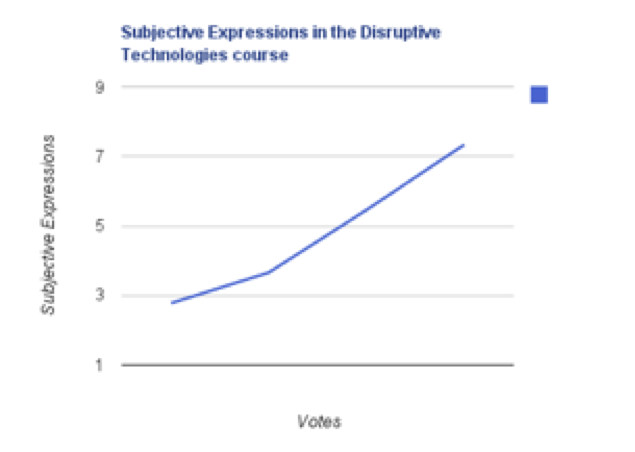
\includegraphics[width = 3.0in, height = 2in]{subjectivity-disrtech.png}
\caption{Subjectivity vs.\ votes.}
\end{center}
\end{figure}

We are interested in modeling engagement and reasoning about which form(s) of engagement are strong indicators of performance. 


%!TEX root = nips2013.tex

\section{Modeling Learner Engagement in PSL}
\label{others}

In this section, we  provide a brief description of PSL. Additional details about PSL are available in \cite{psl}. We also discuss the various features (behavioral, linguistic and structural), which learners exhibit online while attending these courses. We then describe the PSL models to model student behavior which capture these features. We begin with a simple model which predicts performance using only behavioral, linguistic, structural and temporal features and then increase its complexity by including forms of engagement and disengagement as a latent feature.

\subsection{Probabilistic Soft Logic}
\label{sec:psl}

Probabilistic soft logic (PSL) \cite{psl} is a framework for collective, probabilistic reasoning
in relational domains (e.g., personalized medicine and opinion diffusion). PSL uses syntax based on first-order logic as a templating language for continuous graphical models over random variables representing soft truth values.
Like other statistical relational learning methods \cite{srl-book}, PSL uses weighted rules to model the dependencies in a domain. However, one distinguishing aspect is that PSL uses continuous variables to represent truth values, relaxing Boolean truth values to the interval [0,1]. Triangular norms, which are continuous relaxations of logical connectives AND
and OR, are used to combine the atoms in the first-order clauses. 
As a result of the soft formulation and the triangular norms, the underlying probabilistic model is a \emph{hinge-loss Markov random field} HL-MRF \cite{bach-uai13}.  
Inference in HL-MRFs is a convex optimization problem, which makes working with PSL very efficient in comparison to relational modeling tools that use discrete representations.

HL-MRFs admit various learning algorithms for fully-supervised training data, and are amenable to point-estimate ``hard'' expectation maximization for partially-supervised data with latent variables \cite{bach-inferning13}. In our model, we exploit this to represent student engagement as a latent variable.

\subsection{Features}
\label{sec:features}
Our PSL model is built on a foundation of observable features from the data. In the following, we detail the various features we collect from the data. Following the first-order logic based syntax of PSL, we describe these features as logical predicates.

\paragraph{Behavioral Features}

Our behavioral features are attributes that the learner exhibits while on the MOOC website. In our models, we consider two types of behavioral features: aggregate and non-aggregate. The aggregate features give the overall behavioral metrics, while the non-aggregate features are at the instance level. The predicates \textit{postActivity}(USER) and \textit{voteActivity}(USER) capture how active the user is in the forums. These are calculated for each user by assessing whether the user posts more than the average number of posts generated by all users. Predicate \textit{reputation}(USER) represents whether the overall reputation of a user is above average. Predicate \textit{posts}(USER, POST) and  \textit{votes}(USER, POST) capture an instance-level log of users posting and voting on the discussion forums. Predicate \textit{upvote}(POST) is true if the post has positive votes and false otherwise, and predicate \textit{downvote}(POST) is true if a post has been downvoted. 

\paragraph{Linguistic Features}
The subjectivity and polarity scores of the posts are from \emph{OpinionFinder} \cite{opinionfinder}, represented by \textit{subjective}(POST) and \textit{polarity}(POST) respectively. Both these predicates are calculated by normalizing the number of subjective/objective tags and positive and negative polarity tags marked by opinion finder.

\paragraph{Temporal Features}
The course is divided into the following time periods: one time period before the course starts and three time periods during the course. The time period splits during the course are constructed according to the deadlines in the course---one before the first assignment, second and third being before and after the midterm respectively. The temporal features \textit{lastQuiz}, \textit{lastLecture}, \textit{lastPost}, \textit{lastView} and \textit{lastVote} capture the time-period in which each last interaction of the user occurred. These features measure to what lengths the user participated in different aspects of the course.

\paragraph{Structural Features}
We also include structural features induced by forum structure. These are given by \textit{sameThread}(POST\_1, POST\_2) and \textit{sameForum}(THREAD\_1, THREAD\_2) to capture posts in the same thread and threads in the same forum respectively. Including these relationships allows for our model to capture structural phenomena in interactions and how it can affect student engagement and performance.

\subsection{PSL Models}
\label{sec:pslmodels}
We now construct two different PSL models for predicting learner performance in a MOOC setting---1) simple model that directly infers learner performance from observable features and 2) latent variable model that infers student engagement as a hidden variable to predict learner performance.

In our simple PSL model, we model performance of user by using the observable behavioral features exhibited by the learner, linguistic features corresponding to the content of the post and structural features derived from forum interaction. Meaningful combinations of one or more observable behavioral features described in Section \ref{sec:features} are used to predict \emph{performance}. Table \ref{table:simplepslmodel} gives a subset of rules used in this model (\emph{U} and \emph{P} in tables \ref{table:simplepslmodel} and \ref{table:latentpslmodel} refer to USER and POST respectively). As can be seen, the observable features directly imply performance of the learner in the simple model.

%\begin{align*}
%w_1 : postActivity(USER) \wedge reputation(USER) \rightarrow performance(USER)\\
%w_2 : voteActivity(USER) \wedge reputation(USER) \rightarrow performance(USER) \\
%w_3 : posts(USER, POST) \wedge positive(POST) \rightarrow performance(USER) \\
%w_4 : posts(USER, POST) \wedge subjective(POST) \rightarrow performance(USER)\\
%w_5 : posts(USER, POST) \wedge upvote(POST) \rightarrow performance(USER)\\
%w_6 : posts(USER_1, POST_1) \wedge performance(USER_1) \wedge sameThread(USER_1) \rightarrow performance(USER_2)
%\end{align*}

%\begin{table}
%\tiny{
%\begin{center}
%	\begin{tabular}{ | l | p{8 cm}| l |p{5cm} | }
%    \hline
%    Weights  &  Rules (Model 1) & Rules (Model 2)\\ \hline
%$w_1$ &  $postActivity(USER) \wedge reputation(USER) \rightarrow performance(USER) $ & $ postActivity(USER) \wedge reputation(USER) \rightarrow eActive(USER)$\\
%$w_2$  & $voteActivity(USER) \wedge reputation(USER) \rightarrow performance(USER)$ &  $voteActivity(USER) \wedge reputation(USER) \rightarrow ePassive(USER)$ \\
%$w_3$ & $posts(USER, POST) \wedge positive(POST) \rightarrow performance(USER)$ &  $ posts(USER, POST) \wedge positive(POST) \rightarrow eActive(USER)$ \\
%$w_4$ & $votes(USER, POST) \wedge positive(POST) \rightarrow performance(USER)$ & $votes(USER, POST) \wedge positive(POST) \rightarrow ePassive(USER)$\\
%$w_5$ & $posts(USER, POST) \wedge upvote(POST) \rightarrow performance(USER)$ &  $posts(USER, POST) \wedge upvote(POST) \rightarrow eActive(USER)$\\
%    \hline
%    \end{tabular}
%    \end{center}
%      \caption{PSL models}
%                    %\vspace{-1.0cm}
%  \label{table:notations}
%}
%\end{table}

We can enhance this type of model by adding latent variables that have semantic meaning but can not be directly measured from the data. We treat learner engagement as a latent variable and associate the various observed features to one or more forms of engagement and use this to predict learner performance. The latent variables in this model are represented by predicates \textit{engagement\_active}, \textit{engagement\_passive} and \textit{disengagement}. In this model, some of the observable features---\emph{postActivity}, voteActivity, viewActivity are used to classify learners into one or more forms of engagement or disengagement. Then the engagement predicates---\textit{engagement\_active}, \textit{engagement\_passive} and \textit{disengagement} conjuncted with features that were not used in classifying user engagement like \emph{reputation} are then used to predict learner performance. Some rules from this model are given in Table \ref{table:latentpslmodel}.

%\textbf{Bert: This model description seems incomplete. What are the rules that imply performance? Are there constraints on the latent variables now? Both cases need pointers from the text to the tables, or if they are just equation blocks that's not necessary.}
%
%\textbf{Bert: I tried to clean things up, but the model description is odd. There's no need for a table, because adding the weight value doesn't add anything to the discussion. We can just say in text that each rule has its own weight. So I would just type these as a block of equations, like you have in the comments}

Learning a model with latent engagement can suggest which forms of engagement are good indicators of learner performance. The weights of the model are learned by performing hard expectation-maximization with performance as a target variable. The resulting model results in better predictive performance and can provide more insight into MOOC user behavior than a simpler model.

\begin{table}
%\begin{center}
\parbox{.45\linewidth}{
\vspace{1.22cm}
	\begin{tabular}{ ll  }
    \hline
\tiny{$\textit{postActivity}(U) \wedge \textit{reputation}(U) \rightarrow \textit{performance}(U) $ }\\
\tiny{$\textit{voteActivity}(U) \wedge \textit{reputation}[(U) \rightarrow \textit{performance}(U)$ }\\
\tiny{$\textit{posts}(U, P) \wedge \textit{positive}(P) \rightarrow \textit{performance}(U)$ }\\
\tiny{$\textit{votes}(U, P) \wedge \textit{positive}(P) \rightarrow \textit{performance}(U)$ }\\
\tiny{$\textit{posts}(U, P) \wedge \textit{upvote}(P) \rightarrow \textit{performance}(U)$ }\\
    \hline
    \end{tabular}
      \caption{Rules for simple PSL model. }
                    %\vspace{-1.0cm}
  \label{table:simplepslmodel}
}
\parbox{.55\linewidth}{
	\begin{tabular}{ c }
    \hline
\tiny{$ \textit{postActivity}(U) \wedge \textit{reputation}(U) \rightarrow \textit{eActive}(U)$}\\
\tiny{$\textit{voteActivity}(U) \wedge \textit{reputation}(U) \rightarrow \textit{ePassive}(U)$} \\
\tiny{$ \textit{posts}(U, P) \wedge \textit{positive}(P) \rightarrow \textit{eActive}(U)$ }\\
\tiny{$\textit{votes}(U, P) \wedge \textit{positive}(P) \rightarrow \textit{ePassive}(U)$}\\
\tiny{$\textit{posts}(U, P) \wedge \textit{upvote}(P) \rightarrow \textit{eActive}(U)$}\\
\tiny{$\textit{posts}(U_1, P_1) \wedge \textit{posts}(U_2, P_2) \wedge \textit{eActive}(U_1) \wedge \textit{sameThread}(P_1, P_2)$}\\
\tiny{$\rightarrow \textit{eActive}(U_2)$}\\
\tiny{$\textit{eActive}(U) \wedge \textit{ePassive}(P) \rightarrow \textit{performance}(U)$}\\
    \hline
    \end{tabular}
      \caption{\noindent Rules for PSL model with latent variables.}
                    %\vspace{-1.0cm}
  \label{table:latentpslmodel}
}
 %   \end{center}
\end{table}


%\subsection{Model 3}
%In this model, we also take into account the temporal features and capture the observed variables over the various time periods in the course and connections between the variables across time periods.  To do so, the course is partitioned into the following time periods - 1) before course starts, 2) first month of course 3) second month of course and 4) after course ends.
%
%Here we make use of latent variables for engagement and connect them across time periods to see how learners transition between one form of engagement to another and see how that affects course completion.
%
%TODO: rules from white board
%The rules in model 3 are changed to include the latent variable engagement.
%\begin{align*}
%postActivity(USER) \wedge reputation(USER) \rightarrow eActive(USER)\\
%voteActivity(USER) \wedge reputation(USER) \rightarrow ePassive(USER)\\
%posts(USER, POST) \wedge positive(POST) \rightarrow eActive(USER)\\
%votes(USER, POST) \wedge positive(POST) \rightarrow ePassive(USER)\\
%posts(USER, POST) \wedge upvote(POST) \rightarrow eActive(USER)\\
%posts(USER_1, POST_1) \wedge eActive(USER_1) \wedge sameThread(POST_1, POST_2) \rightarrow eActive(USER_2)
%\end{align*}
%!TEX root = sigchi-sample.tex

\section{Experimental Results}
\label{sec:experiments}

We evaluate our models using data from a Coursera course, \emph{Surviving Disruptive Technologies}, taught by Professor Hank Lucas. The seven-week course had 1665 users participating in the forums and 826 users completing the course with a nonzero score. 

We conducted experiments that help us answer the following questions about learner engagement: (1) How effective are our models in predicting performance? (2) What are the key factors influencing learner performance in an online setting? \\

To address the first question, we evaluate the performance of our models in predicting learner \emph{performance}. We use Area under ROC curve (AUC) for our evaluations. We use 10-fold cross-validation in our experiments, leaving out 10\% of the data for testing and rest for training phase, where the model weights are learned. We observe that the PSL model with the latent engagement variables performs better at predicting learner performance and also provides more understanding of reasons why the user did not perform. Table \ref{table:results} shows the AUC values for the PSL models discussed in Section \ref{sec:pslmodels}.

\begin{table} [ht]
\begin{tabular}{ccccc}
\toprule
& AUC-PR Pos. & AUC-PR Neg.& AUC-ROC & Kendall \\
\midrule
Simple PSL Model & 0.7323 & 0.5369 &0.6545 & 0.6545 \\
PSL Model with Latent Variables &0.7506 & 0.5443 & 0.6755 &0.5660 \\
\bottomrule
\end{tabular}
\caption{Performance of simple PSL model and PSL model with latent variables.}
\label{table:results}
\end{table}

To address the second question, we examined weights our model learns for the different engagement variables in predicting performance. We see that the rules involving predicates -- \emph{postActivity}, \emph{voteActivity}, \emph{viewActivity} and \emph{reputation} gain a high weight in the simple learned model. In our second model, we observe that rules involving \emph{engagement\_active} predicts performance, while rules containing \emph{disengagement} gain a higher weight in predicting \emph{$\neg$ performance}.

In addition to predicting performance, the engagement variables are helpful in interpreting the different facets of learner participation in the course. Of particular interest is the content of the posts made by learners and how it corresponds to the values predicted by the our model. Table \ref{table:examples} shows some examples of posts made by users and the engagement and performance scores predicted by the model. It is interesting to note that engaged learners post content with negative sentiment on the course, which may be perceived as participating in the course, for example, the first user in the Table \ref{table:examples}. While, disengaged learners may post similar content with negative sentiment, but a change in activity will help discern them from the engaged ones, e.g., the third user in Table \ref{table:examples}. 

\begin{table} [ht]
\begin{center}
	\begin{tabular}{ p{1.75cm}p{2cm}p{9cm} }
    \toprule
\tiny{Engaged learner \newline (positive sentiment)} & \tiny{performance = 0.7508 \newline disengagement = 1.0} & \tiny{Prof. Lucas, Thank you for a great course! And thank you Coursera!} \\
\tiny{Engaged learner \newline (negative sentiment)} & \tiny{performance = 0.8032 \newline disengagement = 1.0} & \tiny{I have also received a 9, the most disappointing thing
is that I have only received good or passing comments from my peers, 3 of 5 did
not post any comment about my work.}\\
\tiny{Disengaged Learner \newline (negative sentiment)} & \tiny{performance = 0.5 \newline disengagement = 0.675} &\tiny{I agree completely. I used a lot of time on my assignment and got 7.5.  think the evaluation criteria were wrong, it shouldn't be rated on whether you have 3 or 4 innovations in your description but on a subjective measure (which is also flawed). Generally you should pass if it's obvious that you have followed the course and that you have tried to use the theories that the course has(to a certain degree ofc.).}\\
\tiny{Disengaged Learner \newline (negative sentiment)} & \tiny{performance = 0.327 \newline disengagement = 1.0} &\tiny{The grades I received are ridiculous! One pointed out that the good point in my assignment was my fluency in English!!! Oh God!Another one told me that I used "general knowledge" for asking the questions. Yes, I've tried to use "general knowledge" for applying the theory so that it is useful (and not just a theory!).I've re-read my assignment and I still can't believe in my grade. Is it really fair?.}\\
\tiny{Auditor} & \tiny{performance = 0.0 \newline disengagement = 1.0}& \tiny{This has been an otherwise fantastic course. Too bad the potential for success is so heavily weighted on two assignments.}\\
    \bottomrule
    \end{tabular}
    \end{center}
      \caption{Relevant forum content posted by users assigned different engagement labels by our model.}
                    %\vspace{-1.0cm}
  \label{table:examples}
\end{table}

%!TEX root = nips2013.tex
\section{Discussion}
\label{sec:disc}
In this work we took a first step towards understanding student engagement and its impact on student performance using data-driven methods. We formalize, using PSL, our intuition that student engagement can be modeled as a complex interaction of behavioral, linguistic and social cues, and show that our model can construct an interpretation for the latent engagement types from data, without supervision, based on their impact on final performance. 

In addition to our empirical results, we provide some qualitative results of possible uses of the learned engagement-classes. While not comprehensive, it demonstrates the direction of our future work---facilitating instructors' intervention when needed, based on identifying user groups and the sentiment emerging from their forum content.




\begin{thebibliography}{1}
\bibitem{psl}
Broecheler, M., Mihalkova, L. \& Getoor, L.,
  Probabilistic Soft Logic.
In {\it Conference on Uncertainty in Artificial Intelligence}, 2010.

\bibitem{kuh}
 Kuh, G. D.,
What we're learning about student engagement from NSSE: Benchmarks for effective educational practices.
{\it Change: The Magazine of Higher Learning}, 2003.

\bibitem{carini}
Carini, R. M., Kuh, G. D. \& Klein, S. P.,
Student engagement and student learning: Testing the linkages.
{\it Research in Higher Education, 47(1), 1-32}, 2006.

\bibitem{kizilcec}
Kizilcec, R. F., Piech, C. \& Schneider, E.,
Deconstructing disengagement: analyzing learner subpopulations in massive open online courses.
In {\it International Conference on Learning Analytics and Knowledge}, 2013.

\bibitem{srl-book}
Getoor, L. \& Tasker, B.,
  Introduction to Statistical Relational Learning.
{\it The MIT Press}, 2007.

\bibitem{opinionfinder}
Wilson, T., Hoffmann, P., Somasundaran, S., Kessler, J., Wiebe, J., Choi, Y., Cardie, C., Riloff, E., \& Patwardhan, S.,
OpinionFinder: A System for Subjectivity Analysis.
In {\it Proceedings of
Human Language Technologies Conference/Conference on Empirical Methods
in Natural Language Processing (HLT/EMNLP 2005), Companion
	Volume (software demonstration)}, 2005.
	
\bibitem{bach-uai13}
Bach, S. H., Huang, B., London, B. \& Getoor, L.,
Hinge-loss Markov Random Fields: Convex Inference for Structured Prediction.
In {\it Uncertainty in Artificial Intelligence}, 2013.

\bibitem{bach-nips12}
Bach, S. H., Broecheler, M., Getoor, L. \& O'Leary, D. P.,
Scaling MPE Inference for Constrained Continuous Markov Random Fields.
In {\it Advances in Neural Information Processing Systems (NIPS) pages 2663--2671}, 2012.

\bibitem{bach-inferning13}
Bach, S. H., Huang, B. \& Getoor, L,
Learning Latent Groups with Hinge-loss Markov Random Fields.
In {\it Inferning: ICML Workshop on Interactions between Inference and Learning}, 2013.

\end{thebibliography} 

% Balancing columns in a ref list is a bit of a pain because you
% either use a hack like flushend or balance, or manually insert
% a column break.  http://www.tex.ac.uk/cgi-bin/texfaq2html?label=balance
% multicols doesn't work because we're already in two-column mode,
% and flushend isn't awesome, so I choose balance.  See this
% for more info: http://cs.brown.edu/system/software/latex/doc/balance.pdf
%
% Note that in a perfect world balance wants to be in the first
% column of the last page.
%
% If balance doesn't work for you, you can remove that and
% hard-code a column break into the bbl file right before you
% submit:
%
% http://stackoverflow.com/questions/2149854/how-to-manually-equalize-columns-
% in-an-ieee-paper-if-using-bibtex
%
% Or, just remove \balance and give up on balancing the last page.
%
\balance

\section{References format}
References must be the same font size as other body text.
% REFERENCES FORMAT
% References must be the same font size as other body text.

\bibliographystyle{acm-sigchi}
\bibliography{sample}
\end{document}
